\section{Spatial Patterns of Heavy Rainfall Clustering}
The purpose of this section is to elucidate the spatial patterns of precipitation that produce a high degree of clustering. 
We first consider how clustering changes in interannual variability 
before we investigate the spatial patterns associated with strong increases in clustering with warming across the CMIP6 ensemble.

Figure \ref{spatial_preference_obsMAP} shows the regression of monthly anomalies in the frequency of occurrence of heavy precipitation, $C$, 
onto the mean area of heavy precipitation features, $A_m$, 
for the observations. 
When tropical precipitation is observed to be highly clustered on the large scale, heavy precipitation tends to occur more frequently in the central equatorial Pacific. 
Figure \ref{spatial_preference_obsMAP} is calculated for all months, 
but similar spatial patterns can be seen in individual months, 
strongest in DJF (Figure S5 in the supporting information). 
Other notable spatial characteristics of the regression include a decrease in heavy precipitation over the maritime continent 
and a small but statistically significant (crosses) decrease in heavy precipitation over the Amazon and Atlantic. 

To quantify the shift of heavy precipitation to the central equatorial Pacific, we define the distance metrics 
$C_z$, which represents the mean distance of heavily precipitating points within the tropics to the meridian given by the longitude 180$^\circ{}$E, 
and $C_m$, which represents a similar metric defined based on distance to the equator. 
These are somewhat arbitrary zonal and meridional reference lines with which to describe the zonal and meridional shifts, 
and the clustering redistribution of heavy precipitation may be better characterized relative to the climatological distribution. 
For example, in most models, with warming heavy precipitation moves south relative to the northern hemisphere climatological convergence zone or north relative the climatological SPCZ or both. 
However, for simplicity, we use $C_z$ and $C_m$ defined based on 180$^\circ{}$E and the equator.

As expected from the regression map, there is a strong relationship between the mean area of features, $A_m$, and $C_z$ (Figure S2 in the supporting information). 
However, as shown in Figure \ref{spatial_preference_obsSCATTER}a, there is also a strong observed relationship in interannual variability between $A_m$ and the total area fraction of heavy precipitation, $A_f$ [$r^2(A_f, A_m) \sim 0.7$], 
with greater $A_f$ favoring greater $A_m$. 
This suggests a large part of the observed regression pattern is due to the effect of changes in the total precipitating area, 
rather than a pure spatial redistribution of a fixed number of heavily precipitating points. 
This complicates the interpretation of increased clustering in internal variability, since when comparing climates, the mean area fraction of heavy precipitation $\overline{A_f}$ remains fixed at 0.05. 
To address this, we estimate the variations in the distribution of heavy precipitation that contribute to variations in $A_m$ independent of changes in $A_f$ using Pearson partial corelation (see Methods).

Both $C_z$ and $C_m$ are negatively correlated with the mean area of heavy precipitation features, $A_m$, when the effect of changes in the area fraction of heavy precipitation, $A_f$, is removed (star in Figure \ref{spatial_preference_obsSCATTER}b), 
suggesting that there is a shift of convection toward the equator and the central Pacific when the tropics are highly clustered. 
For a given $A_f$, this contraction of heavily precipitating regions explains about 5-10 percent of the remaining variance after the effect of changes in $A_f$ is removed.

Both the CMIP ensemble and the high-resolution model generally show similar spatial patterns associated with increasing large-scale clustering (Figure \ref{spatial_preference_obsSCATTER}b and Figure S6a-b in the supporting information). 
All models show significant relationships between $A_m$ and $A_f$, although generally somewhat weaker than in observations, 
and most models show significant negative partial correlations between the distance metrics $C_z$ (24/27 CMIP6 models) 
and $C_m$ (22/27 CMIP6 models) 
after removing the effect of changes in $A_f$ (Figure \ref{spatial_preference_obsSCATTER}b). 
That is, as for the observations, most models agree that higher clustering, as measured by a larger mean area of heavy precipitation features, is associated with a shift in convection toward the central equatorial Pacific. 
Interestingly, the high-resolution GCM did not show a significant partial correlation with $C_m$, suggesting clustering in that model is not sensitive to the meridional contraction of heavy precipitation to the equator.

\clearpage
\begin{figure}
    \centering
    \includegraphics{sections/result_1/figures/linear_regression_map_conv.pdf}
    \caption{GPCP frequency of occurrence of heavy precipitation, $C$, 
    regressed onto the mean area of heavy precipitation features, $A_m$, 
    for interannual variability. 
    The contour shows the 90th percentile of the climatological $C$ 
    and crosses indicate whether correlations are statistically significant.}
\label{spatial_preference_obsMAP}
\end{figure}

\begin{figure}
    \centering
    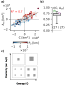
\includegraphics{sections/result_1/figures/scatter_and_box_cz_alt.pdf}    
    \caption{Scatter plot of monthly anomalies in area fraction of heavy precipitation, $A_f$, 
    and the mean area of heavy precipitation features, $A_m$, 
    colored by the zonal proximity of heavy precipitation to the longitude 180$^\circ$ E in the central pacific, $C_z$, 
    for GPCP observations (a). 
    Boxplot of the correlations between $A_f$ and $A_m$ and partial correlations of $C_z$ and the proximity of heavy precipitation to the equator, $C_m$, with $A_m$ 
    outside the influence of $A_f$ 
    for the CMIP6 ensemble (b). 
    The fraction of CMIP models with statistically significant correlations is indicated below each box, 
    and the GPCP (star) 
    and high-resolution GCM (diamond) 
    correlations are shown in lighter colors if not statistically significant.}
\label{spatial_preference_obsSCATTER}
\end{figure}

\begin{figure}
    \centering
    \includegraphics{sections/result_1/figures/cz_cm_cheq_alt.pdf}    
    \caption{Scatter plot of monthly anomalies in area fraction of heavy precipitation, $A_f$, 
    and the mean area of heavy precipitation features, $A_m$, 
    colored by the zonal proximity of heavy precipitation to the longitude 180$^\circ$ E in the central pacific, $C_z$, 
    for GPCP observations (a). 
    Boxplot of the correlations between $A_f$ and $A_m$ and partial correlations of $C_z$ and the proximity of heavy precipitation to the equator, $C_m$, with $A_m$ 
    outside the influence of $A_f$ 
    for the CMIP6 ensemble (b). 
    The fraction of CMIP models with statistically significant correlations is indicated below each box, 
    and the GPCP (star) 
    and high-resolution GCM (diamond) 
    correlations are shown in lighter colors if not statistically significant.}
\label{spatial_preference_obsSCATTER2}
\end{figure}

\clearpage

We now consider how large-scale clustering of heavy precipitation changes under climate change. 
\citet{Blackberg_Singh2022} noted that large-scale clustering increases as the climate warms in projections of climate change by the CMIP5 ensemble. 
Figure \ref{spatial_preference_warmingSCATTER_BOX}a shows that this is also true for CMIP6; 
all models project an increase in $A_m$ with warming to varying degrees. 
However, there is a wide spread in climatological $A_m$ 
and wide spread in climatological increase in $A_m$ across the ensemble, 
suggesting the degree of large-scale clustering and the change in large-scale clustering with warming is poorly constrained in the models. 

Given the climatologically fixed $A_f$ in this framework, changes in the mean area of precipitation features, $A_m$, with warming are driven entirely by a spatial reorganization of convection to larger features. 
The present analysis evaluates whether the spatial patterns associated with a high degree of clustering of precipitation in interannual variability may also be relevant to the redistribution of heavy precipitation causing increased clustering under warming. 
Indeed, all but one model show a reduction in $C_m$ with warming, indicating a contraction of heavy precipitation towards the equator (Figure \ref{spatial_preference_warmingSCATTER_BOX}b). 
Further, all models contract heavy precipitation towards the hydrological equator, or "ITCZ center", 
which is defined here as the latitude of highest specific humidity at 700 hPa as a function of longitude and time in months (Figure \ref{spatial_preference_warmingSCATTER_BOX}c). 
One possible interpretation of this is that a narrowing of the ITCZ provides a mechanism for the overall increase in clustering with warming. 
However, we note that the change in $C_m$ with warming is uncorrelated with the change in $A_m$ across the CMIP6 ensemble; 
models exhibiting stronger ITCZ narrowing with warming do not show stronger increases in large-scale clustering of precipitation. 
On the other hand, there is a significant correlation between increases in mean area of precipitation features, $A_m$, and changes in $C_z$ across the CMIP6 ensemble. 
That is, models that show a greater clustering with warming also show a more zonal shift of heavy precipitation to the central Pacific (note that the zonal and meridional contractions are somewhat anticorrelated, as also identified by \citet{Popp2019}).

Going beyond the simple distance metrics, Figure \ref{spatial_preference_warmingMAP} regresses the projected increase in frequency of occurrence of heavy precipitation onto the projected increase in $A_m$ across the CMIP ensemble. 
This reveals a spatial pattern of precipitation changes with several similarities to the pattern for interannual variability shown in Figure \ref{spatial_preference_obsMAP}. 
However, an important distinction is that, for changes with warming, the redistribution of heavy precipitation is a conserved property, due to the climatologically fixed $A_f$. 
Similarities between the regression patterns include a regression coefficient largest in the central Pacific close to the equator, 
and a redistribution of precipitation away from the maritime continent, Amazon, and Atlantic. 
While under interannual variability heavy precipitation shifts southward in the Pacific for highly clustered states, the changes with warming show a northward shift of heavy precipitation in the Pacific. 

We note that the spatial patterns associated with a climatologically high degree of clustering of heavy precipitation across the CMIP6 ensemble are rather different from those of internal variability and changes with warming (Figure S6c in the supporting information). 
Models with high climatological values of $A_m$ tend to have more convection in the warm pool, over tropical continents, and at the edges of the northern and southern convergence zones over the Pacific Ocean. 
These relationships cannot be summarized by a single value of either $C_z$ or $C_m$. 
Rather, we find that high climatological values of $A_m$ are associated with high month-to-month variability in $A_f$. 
This indicates that high spatial clustering also corresponds to high clustering in time, with some days producing a large amount of heavy precipitation across the tropics and other days producing much less.

\clearpage
\begin{figure}
    \centering
    \includegraphics{sections/result_1/figures/linear_regression_change_conv.pdf}
    \caption{Scatter plot of change in climatological mean area of heavy precipitation features, $A_m$, with change in climatological mean distance of heavy precipitation to the central pacific, $C_z$, (a) and change in mean heavy precipitation proximity to the equator, $C_m$ (b). Boxplot of change in climatological mean distance to the hydrological equator, $C_{heq}$, (c) where the hydrological equator is defined as the latitude of highest specific humidity at 700 hPa as a function of longitude and time in months. All quantities are normalized by the tropical surface temperature warming from the historical to the SSP585 scenario simulation period in CMIP6 models.}
\label{spatial_preference_warmingSCATTER_BOX}
\end{figure}

\begin{figure}
    \centering
    \includegraphics{sections/result_1/figures/clim_change_scatter_cz_cm_cheq}
    \caption{Increase in frequency of occurrence of heavy precipitation, $C$, regressed onto increase in $A_m$ per kelvin tropical warming from the historical to the SSP585 scenario simulation period across the CMIP6 ensemble. Contour shows the ensemble-mean 90th percentile of $C$ in the historical period and crosses indicate whether correlations are statistically significant.}
\label{spatial_preference_warmingMAP}
\end{figure}
\clearpage

In summary, the spatial patterns of heavy precipitation associated with highly clustered states vary across timescales, but there are important common threads. 
In both internal variability and for changes with warming, higher clustering as measured by $A_m$ is associated with more heavy precipitation in the central equatorial Pacific. 
In particular, models with stronger increases in large-scale clustering of precipitation under warming also exhibit greater zonal shifts in convection to the central Pacific. 
This potentially suggests the Walker circulation, and the East-West SST gradient in the Pacific, as an important control on the magnitude of changes in large-scale clustering of precipitation with warming. 
We next investigate the relationships between SST changes and changes in $A_m$ in both internal variability and under climate change.










